\documentclass{article}

% content/resources/templates/preamble.tex
\usepackage[margin=0.6in]{geometry}
\author{Milav Dabgar}
\usepackage{amsmath,amssymb,amsthm}
\usepackage{booktabs}
\usepackage{multirow}
\usepackage{xcolor}
\usepackage{tcolorbox}
\tcbuselibrary{breakable,skins}
\usepackage[colorlinks=true,linkcolor=blue]{hyperref}
\usepackage{titlesec}
\usepackage{enumitem}
\usepackage{tikz}
\usepackage{pgfplots}
\usepackage{circuitikz}
\usepackage[version=4]{mhchem}
\usepackage{longtable}
\usepackage{array}
\usepackage{float}
\usepackage{caption}
\usepackage{listings}

\lstset{
  basicstyle=\small\ttfamily,
  breaklines=true,
  breakatwhitespace=false,
  postbreak=\mbox{\textcolor{red}{$\hookrightarrow$}\space},
  float=false,
  numbers=left,
  numberstyle=\tiny\color{gray},
  numbersep=10pt,
  xleftmargin=2em,
  keywordstyle=\color{blue},
  commentstyle=\color{green!60!black},
  stringstyle=\color{purple},
  backgroundcolor=\color{gray!5},
  showstringspaces=false,
  tabsize=2,
  captionpos=b,
  keepspaces=true,
  columns=flexible
}

\pgfplotsset{compat=1.18}
\usetikzlibrary{shapes,arrows,positioning,calc,patterns,decorations.pathmorphing,decorations.markings,arrows.meta}

% Color scheme
\definecolor{headcolor}{RGB}{0,102,204}
\definecolor{keycolor}{RGB}{220,20,60}
\definecolor{solutioncolor}{RGB}{34,139,34}
\definecolor{mnemoniccolor}{RGB}{148,0,211}
\definecolor{codecolor}{RGB}{0,0,100}

% Spacing
\setlength{\parskip}{3pt}
\setlist[itemize]{nosep}
\setlist[enumerate]{nosep}

% Title formatting
\titleformat{\section}{\Large\bfseries\color{headcolor}}{\thesection}{1em}{}
\titleformat{\subsection}{\large\bfseries\color{headcolor}}{\thesubsection}{1em}{}

% Pandoc tightlist compatibility
\providecommand{\tightlist}{%
  \setlength{\itemsep}{0pt}\setlength{\parskip}{0pt}}

% Pandoc longtable compatibility
\newcounter{none}
\def\thenone{}


% content/resources/templates/english-boxes.tex

% Custom environments
\newtcolorbox{solutionbox}{
 breakable,
 enhanced,
 colback=solutioncolor!5!white,
 colframe=solutioncolor!75!black,
 fonttitle=\bfseries,
 title=Solution
}

\newtcolorbox{solutionboxnobreak}{
 colback=solutioncolor!5!white,
 colframe=solutioncolor!75!black,
 fonttitle=\bfseries,
 title=Solution
}

\newtcolorbox{keyformula}{
 breakable,
 enhanced,
 colback=keycolor!5!white,
 colframe=keycolor!75!black,
 fonttitle=\bfseries,
 title=Key Formula
}

\newtcolorbox{mnemonicboxenv}{
 breakable,
 enhanced,
 colback=mnemoniccolor!5!white,
 colframe=mnemoniccolor!75!black,
 fonttitle=\bfseries,
 title=Mnemonic
}

\newcommand{\mnemonicbox}[1]{%
  \begin{mnemonicboxenv}
    #1
  \end{mnemonicboxenv}
}


% Custom commands for GTU solutions
% This file defines semantic commands for consistent formatting

% Question command with automatic formatting
\newcommand{\question}[2]{%
  \section*{Question #1}%
  \textbf{#2}%
}

% OR question variant
\newcommand{\questionor}[2]{%
  \section*{Question #1 OR}%
  \textbf{#2}%
}

% Proper table environment with caption
\newenvironment{answertable}[1]{%
  \begin{table}[htbp]
  \centering
  \caption{#1}
}{%
  \end{table}
}

% Proper figure environment for diagrams
\newenvironment{answerdiagram}[1]{%
  \begin{figure}[htbp]
  \centering
  \caption{#1}
}{%
  \end{figure}
}

% Semantic markup for key terms
\newcommand{\keyword}[1]{\textbf{#1}}
\newcommand{\code}[1]{\texttt{#1}}
\newcommand{\classname}[1]{\texttt{#1}}
\newcommand{\methodname}[1]{\texttt{#1}}

% Proper quotation marks
\newcommand{\mnemonic}[1]{``#1''}


\title{Antenna and Wave Propagation (4341106) - Summer 2023 Solution}
\date{July 20, 2023}

\begin{document}
\maketitle

\questionmarks{1(a)}{3}{Write any three properties of Electromagnetic waves}

\begin{solutionbox}
\textbf{Properties of Electromagnetic Waves:}

\begin{tabulary}{\linewidth}{|L|}
\hline
1. EM waves can travel through vacuum or material media \\ \hline
2. EM waves travel at the speed of light in free space ($3 \times 10^8$ m/s) \\ \hline
3. EM waves exhibit transverse wave characteristics with oscillating electric and magnetic fields \\ \hline
\end{tabulary}
\end{solutionbox}

\begin{mnemonicbox}
\mnemonic{"VTS" - Vacuum travel, Transverse nature, Speed of light}
\end{mnemonicbox}

\questionmarks{1(b)}{4}{Define: (1) Radiation resistance (2) Directivity (3) Gain}

\begin{solutionbox}
\textbf{Definitions:}

\begin{tabulary}{\linewidth}{|L|L|}
\hline
\textbf{Term} & \textbf{Definition} \\ \hline
\keyword{Radiation resistance} & The equivalent resistance that would dissipate the same amount of power as radiated by an antenna when the current at the feed point is equal to the antenna input current \\ \hline
\keyword{Directivity} & The ratio of maximum radiation intensity in a specific direction to the average radiation intensity in all directions \\ \hline
\keyword{Gain} & The product of directivity and radiation efficiency, measuring how efficiently an antenna converts input power into radio waves in a specific direction \\ \hline
\end{tabulary}
\end{solutionbox}

\begin{mnemonicbox}
\mnemonic{"RDG" - Resistance dissipates power, Direction concentration, Gain includes efficiency}
\end{mnemonicbox}

\questionmarks{1(c)}{7}{Explain physical concept of generation of Electromagnetic waves with neat diagram}

\begin{solutionbox}
Electromagnetic waves are generated when electric charges accelerate or oscillate, creating coupled oscillating electric and magnetic fields that propagate through space.

\begin{center}
\begin{tikzpicture}[node distance=2cm, auto]
    \node [gtu block] (curr) {Electric Current Flow};
    \node [gtu block, right=of curr] (elec) {Oscillating Electric Field};
    \node [gtu block, below=of elec] (mag) {Oscillating Magnetic Field};
    \node [gtu block, right=of elec] (prop) {Self-sustaining wave propagation};

    \draw [gtu arrow] (curr) -- node {Oscillation} (elec);
    \draw [gtu arrow] (elec) -- node {Induces} (mag);
    \draw [gtu arrow] (mag) -- node [left] {Induces} (elec);
    \draw [gtu arrow] (elec) -- (prop);
\end{tikzpicture}
\end{center}

\begin{answerdiagram}{Dipole Antenna EM Wave Generation}
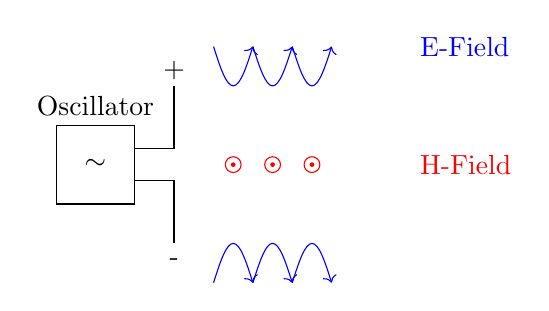
\begin{tikzpicture}[scale=1]
    % Dipole
    \draw [thick] (0, 1) -- (0, 0.2);
    \draw [thick] (0, -1) -- (0, -0.2);
    \node at (0, 1.2) {+};
    \node at (0, -1.2) {-};
    
    % Source
    \draw (-0.5, 0.2) -- (0, 0.2);
    \draw (-0.5, -0.2) -- (0, -0.2);
    \draw (-0.5, -0.5) rectangle (-1.5, 0.5);
    \node at (-1, 0) {$\sim$};
    \node [above] at (-1, 0.5) {Oscillator};

    % E-field
    \foreach \x in {1, 2, 3} {
        \draw [blue, ->] (0.5*\x, 1.5) sin (0.5*\x+0.25, 1) cos (0.5*\x+0.5, 1.5);
        \draw [blue, ->] (0.5*\x, -1.5) sin (0.5*\x+0.25, -1) cos (0.5*\x+0.5, -1.5);
    }
    \node [blue, right] at (3, 1.5) {E-Field};

    % H-field (circles)
    \foreach \x in {1, 2, 3} {
        \draw [red] (0.5*\x + 0.25, 0) circle (0.1);
        \fill [red] (0.5*\x + 0.25, 0) circle (0.03);
    }
    \node [red, right] at (3, 0) {H-Field};
\end{tikzpicture}
\end{answerdiagram}

\begin{itemize}
    \item \textbf{Basic concept}: When AC current flows in the antenna, electrons accelerate up and down.
    \item \textbf{Electric field}: Created by charge separation in the antenna.
    \item \textbf{Magnetic field}: Produced by the current flow, perpendicular to electric field.
    \item \textbf{Propagation}: Fields detach from antenna and propagate outward at the speed of light.
    \item \textbf{Self-sustaining}: Each field component regenerates the other as wave travels.
\end{itemize}
\end{solutionbox}

\begin{mnemonicbox}
\mnemonic{"COMAP" - Current Oscillations Make Alternating Propagations}
\end{mnemonicbox}

\orquestionmarks{1(c)}{7}{Design 4 Element Yagi Uda antenna for frequency of 435 MHz with necessary equations}

\begin{solutionbox}
\textbf{Design for 435 MHz 4-Element Yagi-Uda Antenna:}

\textbf{Equations used}:
\begin{itemize}
    \item Wavelength: $\lambda = c/f = 3\times10^8 / 435\times10^6 = 0.69$ meters
    \item Half-wave dipole: $L = 0.5\lambda = 34.5$ cm
    \item Element spacing: $S = 0.15\lambda$ to $0.25\lambda$
\end{itemize}

\textbf{Calculated Values:}
\begin{tabulary}{\linewidth}{|L|L|L|L|}
\hline
\textbf{Element} & \textbf{Length Formula} & \textbf{Spacing Formula} & \textbf{Value} \\ \hline
\textbf{Reflector} & $0.5\lambda \times 1.05$ & - & 36.2 cm \\ \hline
\textbf{Driven element} & $0.5\lambda$ & - & 34.5 cm \\ \hline
\textbf{Director 1} & $0.45\lambda$ & $0.2\lambda$ from driven & 31.0 cm (Sp: 13.8 cm) \\ \hline
\textbf{Director 2} & $0.43\lambda$ & $0.25\lambda$ from D1 & 29.6 cm (Sp: 17.2 cm) \\ \hline
\end{tabulary}

\begin{answerdiagram}{4-Element Yagi-Uda Antenna Layout}
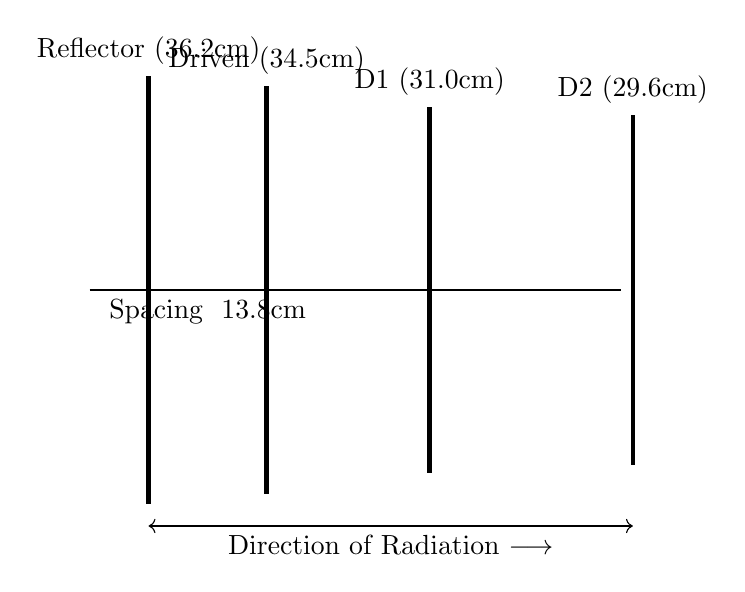
\begin{tikzpicture}[scale=0.15]
    % Boom
    \draw [thick] (-5, 0) -- (40, 0);
    
    % Elements (vertical lines centered on boom)
    % Reflector
    \draw [ultra thick] (0, -18.1) -- (0, 18.1) node [above] {Reflector (36.2cm)};
    
    % Driven
    \draw [ultra thick] (10, -17.25) -- (10, 17.25) node [above] {Driven (34.5cm)};
    \node [below] at (5, 0) {Spacing ~13.8cm}; % Approx spacing visual
    
    % Director 1
    \draw [ultra thick] (23.8, -15.5) -- (23.8, 15.5) node [above] {D1 (31.0cm)};
    
    % Director 2
    \draw [ultra thick] (41, -14.8) -- (41, 14.8) node [above] {D2 (29.6cm)};
    
    \draw [<->] (0, -20) -- (41, -20) node [midway, below] {Direction of Radiation $\longrightarrow$};
\end{tikzpicture}
\end{answerdiagram}
\end{solutionbox}

\begin{mnemonicbox}
\mnemonic{"RDDS" - Reflector Driven Directors Shrink}
\end{mnemonicbox}

\questionmarks{2(a)}{3}{Explain Loop antenna with diagram}

\begin{solutionbox}
Loop antenna is a radiating element formed by shaping a conductor into a loop.

\begin{answerdiagram}{Loop Antenna}
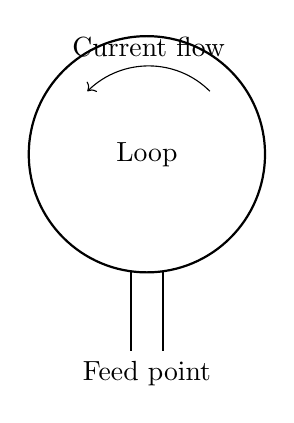
\begin{tikzpicture}
    \draw [thick] (0,0) circle (1.5cm);
    \draw [->] (0.8, 0.8) arc (45:135:1.1) node [midway, above] {Current flow};
    \draw [thick] (-0.2, -1.5) -- (-0.2, -2.5);
    \draw [thick] (0.2, -1.5) -- (0.2, -2.5);
    \node [below] at (0, -2.5) {Feed point};
    \node at (0,0) {Loop};
\end{tikzpicture}
\end{answerdiagram}

\begin{itemize}
    \item \textbf{Small loops}: Circumference $< \lambda/10$, radiation pattern similar to magnetic dipole.
    \item \textbf{Large loops}: Circumference $\approx$ wavelength, bidirectional radiation pattern.
    \item \textbf{Applications}: Direction finding, AM radio reception, RFID tags.
\end{itemize}
\end{solutionbox}

\begin{mnemonicbox}
\mnemonic{"SLC" - Size affects Loop Characteristics}
\end{mnemonicbox}

\questionmarks{2(b)}{4}{Explain Non Resonant wire antenna}

\begin{solutionbox}
\textbf{Non-Resonant Wire Antenna:}

\begin{tabulary}{\linewidth}{|L|L|}
\hline
\textbf{Characteristic} & \textbf{Description} \\ \hline
\keyword{Definition} & Antenna operating at frequencies where its physical length is not a multiple of half-wavelength \\ \hline
\keyword{Impedance} & Complex with both resistive and reactive components \\ \hline
\keyword{Standing waves} & Present along the antenna length \\ \hline
\keyword{Example} & Rhombic antenna, terminated with resistance at the end \\ \hline
\keyword{Advantage} & Wideband operation, suitable for multiple frequencies \\ \hline
\end{tabulary}
\end{solutionbox}

\begin{mnemonicbox}
\mnemonic{"NITRO" - Non-resonance Incurs Termination for Resistance and Operation}
\end{mnemonicbox}

\questionmarks{2(c)}{7}{What is Radiation resistance of half wave dipole? Draw radiation patterns of Dipoles of length $\lambda/2$, $\lambda$ and $\lambda/4$ antenna}

\begin{solutionbox}
The radiation resistance of a half-wave dipole is approximately \textbf{73 ohms}.

\textbf{Radiation Patterns:}

\begin{answerdiagram}{Dipole Radiation Patterns}
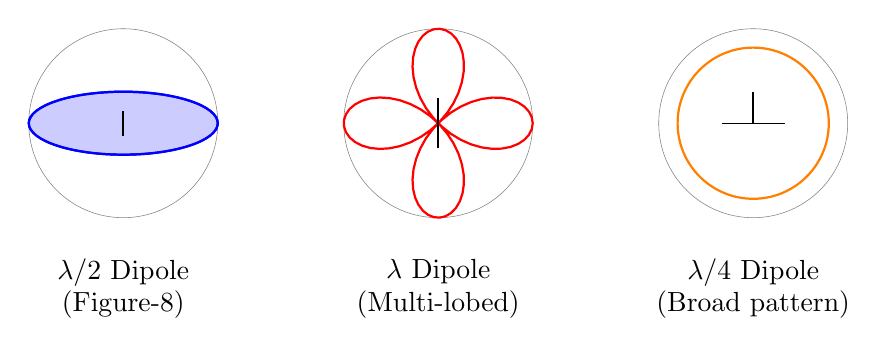
\begin{tikzpicture}[scale=0.8]
    % Lambda/2
    \begin{scope}[xshift=0cm]
        \draw [help lines] (0,0) circle (1.5);
        \draw [thick, blue, rotate=90] (0,0) ellipse (0.5 and 1.5);
        \draw [thick, blue, rotate=90] (0,0) ellipse (0.5 and 1.5); % Figure 8 visual
        \fill [blue, opacity=0.2, rotate=90] (0,0) ellipse (0.5 and 1.5);
        \node [below] at (0, -2) {$\lambda/2$ Dipole};
        \node [below] at (0, -2.5) {(Figure-8)};
        \draw [thick] (0, -0.2) -- (0, 0.2); % Antenna
    \end{scope}

    % Lambda
    \begin{scope}[xshift=5cm]
        \draw [help lines] (0,0) circle (1.5);
        % Multi-lobed
        \draw [thick, red] plot [domain=0:360, samples=100] ({1.5*cos(2*\x)*cos(\x)}, {1.5*cos(2*\x)*sin(\x)});
        \node [below] at (0, -2) {$\lambda$ Dipole};
        \node [below] at (0, -2.5) {(Multi-lobed)};
        \draw [thick] (0, -0.4) -- (0, 0.4); % Antenna
    \end{scope}

    % Lambda/4
    \begin{scope}[xshift=10cm]
        \draw [help lines] (0,0) circle (1.5);
        \draw [thick, orange] (0,0) circle (1.2); % Omnidirectional-ish / Broad
        \node [below] at (0, -2) {$\lambda/4$ Dipole};
        \node [below] at (0, -2.5) {(Broad pattern)};
        \draw [thick] (0, 0) -- (0, 0.5); % Monopole
        \draw (-0.5, 0) -- (0.5, 0); % Ground
    \end{scope}
\end{tikzpicture}
\end{answerdiagram}

\begin{tabulary}{\linewidth}{|L|L|}
\hline
\textbf{Dipole Length} & \textbf{Pattern Characteristics} \\ \hline
\textbf{$\lambda/2$ dipole} & Figure-8 pattern; maximum radiation perpendicular to antenna axis; HPBW = $78^\circ$ \\ \hline
\textbf{$\lambda$ dipole} & Multi-lobed pattern; four main lobes at angles to antenna axis \\ \hline
\textbf{$\lambda/4$ dipole} & Broader pattern than $\lambda/2$; requires ground plane to complete the equivalent dipole \\ \hline
\end{tabulary}
\end{solutionbox}

\begin{mnemonicbox}
\mnemonic{"SHORT" - Smaller Half-dipole Offers Rounded-Transmissions}
\end{mnemonicbox}

\orquestionmarks{2(a)}{3}{Explain Folded dipole antenna with figure}

\begin{solutionbox}
Folded dipole is a variation of the half-wave dipole with ends folded back and connected to form a loop.

\begin{answerdiagram}{Folded Dipole}
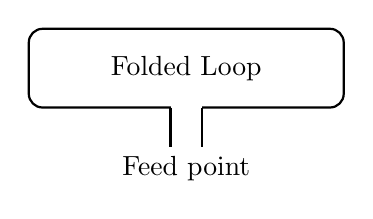
\begin{tikzpicture}
    \draw [thick, rounded corners=5pt] (-2, 0.5) rectangle (2, -0.5);
    \fill [white] (-0.2, -0.6) rectangle (0.2, -0.4); % Break bottom
    \draw [thick] (-0.2, -0.5) -- (-0.2, -1);
    \draw [thick] (0.2, -0.5) -- (0.2, -1);
    \node [below] at (0, -1) {Feed point};
    \node at (0, 0) {Folded Loop};
\end{tikzpicture}
\end{answerdiagram}

\begin{itemize}
    \item \textbf{Input impedance}: Approximately 300 ohms (4 times that of simple dipole).
    \item \textbf{Bandwidth}: Wider than simple dipole.
    \item \textbf{Applications}: TV reception, FM radio, balanced transmission lines.
\end{itemize}
\end{solutionbox}

\begin{mnemonicbox}
\mnemonic{"FIB" - Folded Increases Bandwidth}
\end{mnemonicbox}

\orquestionmarks{2(b)}{4}{Explain Rhombic antenna with figure}

\begin{solutionbox}
Rhombic antenna consists of four wires arranged in a rhombus or diamond shape.

\begin{answerdiagram}{Rhombic Antenna}
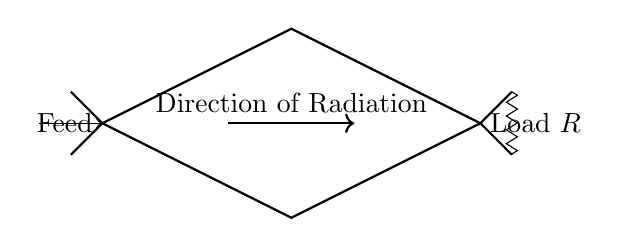
\begin{tikzpicture}[scale=0.8]
    \coordinate (A) at (0,0);
    \coordinate (B) at (3,1.5);
    \coordinate (C) at (6,0);
    \coordinate (D) at (3,-1.5);
    
    \draw [thick] (A) -- (B) -- (C) -- (D) -- cycle;
    
    \draw [->] (-1, 0) -- (0, 0) node [left] {Feed};
    \draw [thick] (A) -- (-0.5, 0.5);
    \draw [thick] (A) -- (-0.5, -0.5);
    
    \node [right] at (C) {Load $R$};
    \draw [thick] (C) -- (6.5, 0.5);
    \draw [thick] (C) -- (6.5, -0.5);
    \draw [decorate, decoration={zigzag, amplitude=2pt, segment length=5pt}] (6.5, 0.5) -- (6.5, -0.5);
    
    \draw [->, thick] (2, 0) -- (4, 0) node [midway, above] {Direction of Radiation};
\end{tikzpicture}
\end{answerdiagram}

\begin{tabulary}{\linewidth}{|L|L|}
\hline
\textbf{Characteristic} & \textbf{Description} \\ \hline
\keyword{Shape} & Diamond/rhombus with terminating resistor at far end \\ \hline
\keyword{Operation} & Non-resonant traveling-wave antenna \\ \hline
\keyword{Directivity} & High gain, unidirectional pattern \\ \hline
\keyword{Bandwidth} & Very wide frequency range \\ \hline
\keyword{Applications} & HF communications, point-to-point links \\ \hline
\end{tabulary}
\end{solutionbox}

\begin{mnemonicbox}
\mnemonic{"TREND" - Terminated Rhombic Enables Numerous Directions}
\end{mnemonicbox}

\orquestionmarks{2(c)}{7}{Differentiate between Broadside array and End fire array with suitable diagram}

\begin{solutionbox}
\textbf{Comparison:}

\begin{tabulary}{\linewidth}{|L|L|L|}
\hline
\textbf{Parameter} & \textbf{Broadside Array} & \textbf{End fire Array} \\ \hline
\keyword{Direction of maximum radiation} & Perpendicular to array axis & Along array axis \\ \hline
\keyword{Element phasing} & Same phase ($0^\circ$) & Progressive phase shift \\ \hline
\keyword{Element spacing} & $\lambda/2$ typically & $\lambda/4$ typically \\ \hline
\keyword{Radiation pattern} & Fan-shaped beam & Pencil-shaped beam \\ \hline
\keyword{Applications} & Broadcasting, base stations & Point-to-point links \\ \hline
\end{tabulary}

\begin{answerdiagram}{Array Comparison}
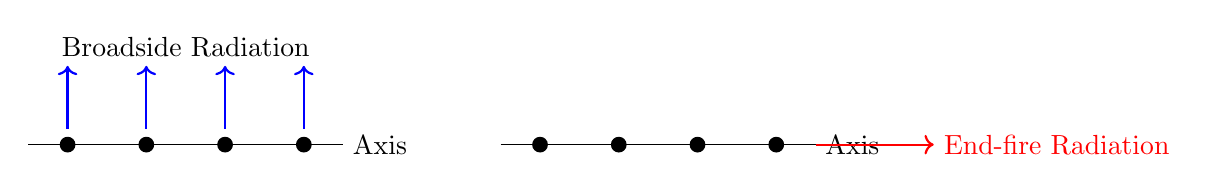
\begin{tikzpicture}
    % Broadside
    \begin{scope}[xshift=0cm]
        \foreach \x in {0,1,2,3} \fill (\x, 0) circle (0.1);
        \draw (-0.5, 0) -- (3.5, 0) node [right] {Axis};
        \foreach \x in {0,1,2,3} \draw [->, thick, blue] (\x, 0.2) -- (\x, 1);
        \node [above] at (1.5, 1) {Broadside Radiation};
    \end{scope}
    
    % End fire
    \begin{scope}[xshift=6cm]
        \foreach \x in {0,1,2,3} \fill (\x, 0) circle (0.1);
        \draw (-0.5, 0) -- (3.5, 0) node [right] {Axis};
        \draw [->, thick, red] (3.5, 0) -- (5, 0) node [right] {End-fire Radiation};
    \end{scope}
\end{tikzpicture}
\end{answerdiagram}
\end{solutionbox}

\begin{mnemonicbox}
\mnemonic{"PAPER" - Perpendicular And Parallel Emission Respectively}
\end{mnemonicbox}

\questionmarks{3(a)}{3}{Draw and Explain Inverted V antenna}

\begin{solutionbox}
Inverted V antenna is a dipole with arms angled downward, resembling an inverted "V".

\begin{answerdiagram}{Inverted V Antenna}
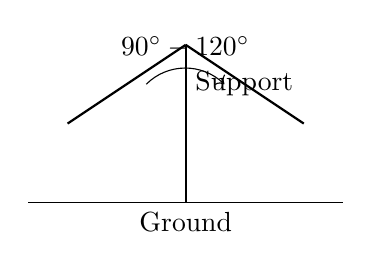
\begin{tikzpicture}
    \draw [thick] (0,0) -- (0, 2); % Support
    \draw [thick] (0, 2) -- (-1.5, 1); % Left arm
    \draw [thick] (0, 2) -- (1.5, 1); % Right arm
    \draw [thick] (0, 2) -- (0, 1.8); % Feed line
    \node [right] at (0, 1.5) {Support};
    \node [below] at (0, 0) {Ground};
    \draw (-2, 0) -- (2, 0);
    \draw [->] (-0.5, 1.5) arc (135:45:0.7) node [midway, above] {$90^\circ - 120^\circ$};
\end{tikzpicture}
\end{answerdiagram}

\begin{itemize}
    \item \textbf{Angle}: Arms typically form $90^\circ-120^\circ$ angle.
    \item \textbf{Impedance}: Close to 50 ohms, lower than horizontal dipole.
    \item \textbf{Pattern}: Omnidirectional, slightly broader than horizontal dipole.
    \item \textbf{Applications}: Amateur radio, shortwave communications.
\end{itemize}
\end{solutionbox}

\begin{mnemonicbox}
\mnemonic{"AVS" - Angle Varies Signal}
\end{mnemonicbox}

\questionmarks{3(b)}{4}{Draw and explain parabolic reflector antenna}

\begin{solutionbox}
\begin{answerdiagram}{Parabolic Reflector Antenna}
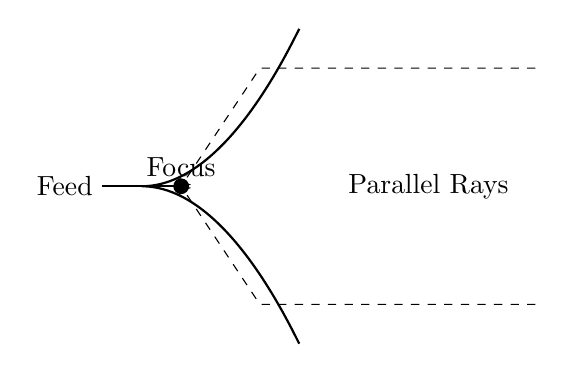
\begin{tikzpicture}
    \draw [thick] (2, 2) parabola bend (0, 0) (2, -2);
    \draw [thick] (-0.5, 0) -- (0.5, 0); % Feed
    \node [left] at (-0.5, 0) {Feed};
    \fill (0.5, 0) circle (0.1) node [above] {Focus};
    \draw [->, dashed] (5, 1.5) -- (1.5, 1.5) -- (0.5, 0); % Incoming ray 1
    \draw [->, dashed] (5, -1.5) -- (1.5, -1.5) -- (0.5, 0); % Incoming ray 2
    \node [right] at (2.5, 0) {Parallel Rays};
\end{tikzpicture}
\end{answerdiagram}

\begin{tabulary}{\linewidth}{|L|L|}
\hline
\textbf{Component} & \textbf{Function} \\ \hline
\keyword{Parabolic reflector} & Collects and focuses incoming signals or directs transmitted signals \\ \hline
\keyword{Feed element} & Located at focal point of parabola to collect/emit signals \\ \hline
\keyword{Focal length} & Distance from vertex to focus, determines beam characteristics \\ \hline
\keyword{Applications} & Satellite communications, radar, radio astronomy, microwave links \\ \hline
\end{tabulary}
\end{solutionbox}

\begin{mnemonicbox}
\mnemonic{"FOLD" - Focus Of Large Dish}
\end{mnemonicbox}

\questionmarks{3(c)}{7}{Write down range of frequencies for HF, VHF and UHF. Write short note on Microstrip antenna.}

\begin{solutionbox}
\textbf{Frequency Ranges:}

\begin{tabulary}{\linewidth}{|L|L|}
\hline
\textbf{Frequency Band} & \textbf{Range} \\ \hline
\textbf{HF (High Frequency)} & 3 MHz - 30 MHz \\ \hline
\textbf{VHF (Very High Frequency)} & 30 MHz - 300 MHz \\ \hline
\textbf{UHF (Ultra High Frequency)} & 300 MHz - 3 GHz \\ \hline
\end{tabulary}

\textbf{Microstrip Antenna:}

\begin{answerdiagram}{Microstrip Antenna Structure}
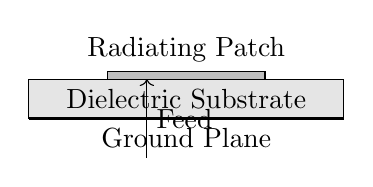
\begin{tikzpicture}
    \draw [fill=gray!20] (0,0) rectangle (4, 0.5); % Substrate
    \draw [fill=gray!50] (1, 0.5) rectangle (3, 0.6); % Patch
    \draw [thick] (0, 0) -- (4, 0); % Ground plane (bottom line)
    \node [below] at (2, 0) {Ground Plane};
    \node at (2, 0.25) {Dielectric Substrate};
    \node [above] at (2, 0.6) {Radiating Patch};
    \draw [->] (1.5, -0.5) -- (1.5, 0.5) node [midway, right] {Feed};
\end{tikzpicture}
\end{answerdiagram}

\begin{itemize}
    \item \textbf{Structure}: Conductive patch on dielectric substrate with ground plane.
    \item \textbf{Feeding methods}: Microstrip line, coaxial probe, aperture-coupled.
    \item \textbf{Advantages}: Low profile, lightweight, easy fabrication, compatible with PCB.
    \item \textbf{Limitations}: Narrow bandwidth, low gain, low power handling.
    \item \textbf{Applications}: Mobile devices, RFID, GPS, satellite communications.
\end{itemize}
\end{solutionbox}

\begin{mnemonicbox}
\mnemonic{"PATCH" - Planar Antenna That's Cheaply Handled}
\end{mnemonicbox}

\orquestionmarks{3(a)}{3}{Write Morse code for word: "LINE OF SIGHT"}

\begin{solutionbox}
\textbf{Morse Code Translation:}

\begin{tabulary}{\linewidth}{|L|L|L|L|}
\hline
\textbf{Letter} & \textbf{Code} & \textbf{Letter} & \textbf{Code} \\ \hline
L & .\,-.. & F & ..-. \\ \hline
I & .. & S & ... \\ \hline
N & -. & G & --. \\ \hline
E & . & H & .... \\ \hline
O & --- & T & - \\ \hline
\end{tabulary}

\textbf{"LINE OF SIGHT"}:
\code{.-.. .. -. . / --- ..-. / ... .. --. .... -}
\end{solutionbox}

\begin{mnemonicbox}
\mnemonic{"Listen In Now, Every Other Frequency Supports Immediate Global Heightened Transmission"}
\end{mnemonicbox}

\orquestionmarks{3(b)}{4}{Draw and explain Turnstile \& Super turnstile antenna}

\begin{solutionbox}
\textbf{Turnstile Antenna:}

\begin{answerdiagram}{Turnstile Antenna}
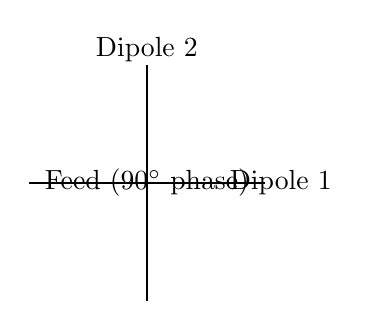
\begin{tikzpicture}
    \draw [thick] (-1.5, 0) -- (1.5, 0);
    \draw [thick] (0, -1.5) -- (0, 1.5);
    \node at (1.7, 0) {Dipole 1};
    \node at (0, 1.7) {Dipole 2};
    \node at (0,0) {Feed (90$^\circ$ phase)};
\end{tikzpicture}
\end{answerdiagram}

\textbf{Super Turnstile Antenna:}
\begin{itemize}
    \item Modification with multiple elements forming rectangular loops (Batwing shape).
    \item Provides broader bandwidth.
\end{itemize}

\begin{tabulary}{\linewidth}{|L|L|}
\hline
\textbf{Type} & \textbf{Characteristics} \\ \hline
\keyword{Turnstile} & Two horizontal dipoles at right angles, fed $90^\circ$ out of phase \\ \hline
\keyword{Super Turnstile} & Uses batwing/sheet elements for wider bandwidth \\ \hline
\keyword{Pattern} & Omnidirectional in horizontal plane, figure-8 in vertical \\ \hline
\keyword{Polarization} & Horizontal or circular polarization \\ \hline
\keyword{Applications} & TV broadcasting, FM broadcasting \\ \hline
\end{tabulary}
\end{solutionbox}

\begin{mnemonicbox}
\mnemonic{"TOPS" - Turnstile Offers Perpendicular Symmetry}
\end{mnemonicbox}

\orquestionmarks{3(c)}{7}{What is Polarization? Explain Helical antenna in detail with diagram}

\begin{solutionbox}
\textbf{Polarization} is the orientation of the electric field vector of an electromagnetic wave as it propagates through space.

\textbf{Helical Antenna:}

\begin{answerdiagram}{Helical Antenna}
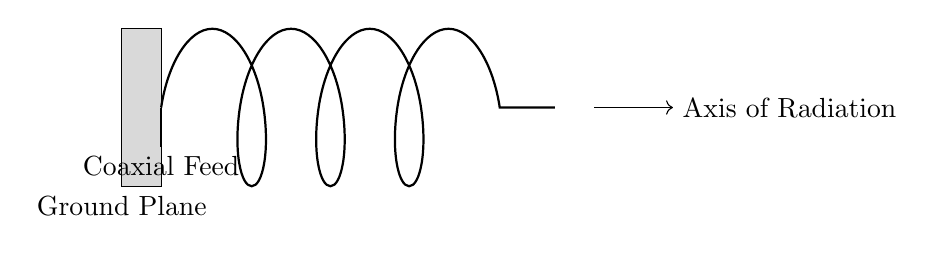
\begin{tikzpicture}[x=1cm, y=0.5cm]
    \draw [fill=gray!30] (0,-2) rectangle (0.5, 2); % Ground plane
    \node [below] at (0, -2) {Ground Plane};
    \draw [thick, decorate, decoration={coil, aspect=0.4, segment length=1cm, amplitude=1cm}] (0.5, 0) -- (5.5, 0);
    \draw [thick] (0.5, 0) -- (0.5, -1); % Coax feed
    \node [below] at (0.5, -1) {Coaxial Feed};
    \draw [->] (6, 0) -- (7, 0) node [right] {Axis of Radiation};
\end{tikzpicture}
\end{answerdiagram}

\begin{tabulary}{\linewidth}{|L|L|}
\hline
\textbf{Parameter} & \textbf{Description} \\ \hline
\keyword{Structure} & Conductor wound in helical shape above ground plane \\ \hline
\keyword{Diameter} & Typically $\lambda/\pi$ \\ \hline
\keyword{Pitch} & Spacing between turns, usually $\lambda/4$ \\ \hline
\keyword{Turns} & 3-10 turns depending on gain requirements \\ \hline
\keyword{Modes} & Normal mode (broadside) or Axial mode (end-fire) \\ \hline
\keyword{Polarization} & Circular polarization in axial mode \\ \hline
\keyword{Applications} & Satellite communications, space telemetry, tracking \\ \hline
\end{tabulary}
\end{solutionbox}

\begin{mnemonicbox}
\mnemonic{"HASP" - Helical Antenna Supports Polarization}
\end{mnemonicbox}

\questionmarks{4(a)}{3}{Explain Tropospheric scattered propagation}

\begin{solutionbox}
\begin{tabulary}{\linewidth}{|L|L|}
\hline
\textbf{Aspect} & \textbf{Description} \\ \hline
\keyword{Mechanism} & Radio signals scatter from tropospheric irregularities and refractive index variations \\ \hline
\keyword{Frequency} & Typically VHF, UHF (100 MHz - 10 GHz) \\ \hline
\keyword{Range} & 100-800 km, beyond line-of-sight \\ \hline
\keyword{Reliability} & Less affected by weather than line-of-sight; more reliable than ionospheric \\ \hline
\keyword{Applications} & Military communications, remote areas \\ \hline
\end{tabulary}
\end{solutionbox}

\begin{mnemonicbox}
\mnemonic{"STRIP" - Scatter Through Refractive Index Patterns}
\end{mnemonicbox}

\questionmarks{4(b)}{4}{Define: (1) Virtual Height (2) Maximum Usable Frequency - MUF (3) Critical Frequency}

\begin{solutionbox}
\begin{tabulary}{\linewidth}{|L|L|}
\hline
\textbf{Term} & \textbf{Definition} \\ \hline
\keyword{Virtual Height} & The apparent height of the ionosphere calculated from the time delay of a radio signal reflected back to Earth, as if reflection occurred at a single point \\ \hline
\keyword{MUF} & The highest frequency that can be used for reliable communication via ionospheric reflection for a specified path and time \\ \hline
\keyword{Critical Frequency} & The highest frequency that can be reflected back when transmitted vertically to the ionosphere (when angle of incidence is 90$^\circ$) \\ \hline
\end{tabulary}
\end{solutionbox}

\begin{mnemonicbox}
\mnemonic{"VMC" - Virtual height Measures Critical reflection}
\end{mnemonicbox}

\questionmarks{4(c)}{7}{Explain effect of ground on electromagnetic wave propagation}

\begin{solutionbox}
\begin{answerdiagram}{Ground Wave Propagation Effects}
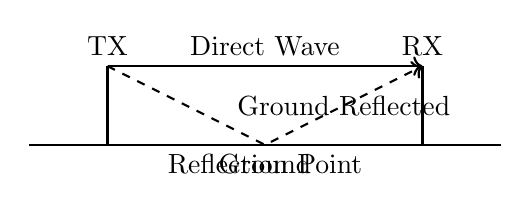
\begin{tikzpicture}
    % Ground
    \draw [thick] (-3, 0) -- (3, 0);
    \node [below] at (0, 0) {Ground};
    
    % TX RX
    \draw [thick] (-2, 0) -- (-2, 1) node [above] {TX};
    \draw [thick] (2, 0) -- (2, 1) node [above] {RX};
    
    % Direct
    \draw [thick, ->] (-2, 1) -- (2, 1) node [midway, above] {Direct Wave};
    
    % Reflected
    \draw [thick, dashed, ->] (-2, 1) -- (0, 0) -- (2, 1);
    \node [below] at (0, 0) {Reflection Point};
    \node at (1, 0.5) {Ground Reflected};
\end{tikzpicture}
\end{answerdiagram}

\begin{tabulary}{\linewidth}{|L|L|}
\hline
\textbf{Effect} & \textbf{Description} \\ \hline
\keyword{Ground reflection} & Signal reflects off ground, causing multipath reception (constructive/destructive interference) \\ \hline
\keyword{Ground absorption} & Part of signal energy absorbed by ground, reducing signal strength \\ \hline
\keyword{Ground diffraction} & Waves bend around obstacles, extending coverage beyond line-of-sight \\ \hline
\keyword{Earth curvature} & Limits line-of-sight distance based on antenna height \\ \hline
\keyword{Ground conductivity} & Higher conductivity (water) allows better propagation than poor conductors (dry soil) \\ \hline
\end{tabulary}

\textbf{Range Equation:} $d \approx 4.12(\sqrt{h_t} + \sqrt{h_r})$ km.
\end{solutionbox}

\begin{mnemonicbox}
\mnemonic{"RADAR" - Reflection Absorption Diffraction Affect Range}
\end{mnemonicbox}

\orquestionmarks{4(a)}{3}{Explain Duct Propagation}

\begin{solutionbox}
Duct propagation occurs when radio waves become trapped in atmospheric layers with special refractive properties.

\begin{answerdiagram}{Atmospheric Duct}
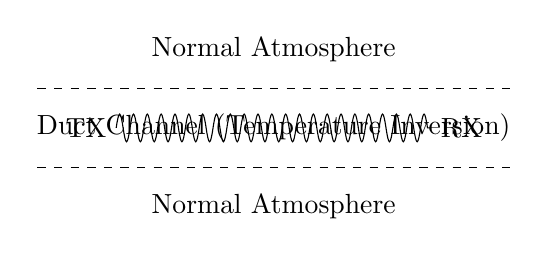
\begin{tikzpicture}
    \draw [dashed] (0, 2) -- (6, 2);
    \draw [dashed] (0, 1) -- (6, 1);
    \node at (3, 1.5) {Duct Channel (Temperature Inversion)};
    \draw [decorate, decoration={coil, aspect=0, segment length=5pt, amplitude=5pt}] (1, 1.5) -- (5, 1.5);
    \node [left] at (1, 1.5) {TX};
    \node [right] at (5, 1.5) {RX};
    \node at (3, 0.5) {Normal Atmosphere};
    \node at (3, 2.5) {Normal Atmosphere};
\end{tikzpicture}
\end{answerdiagram}

\begin{itemize}
    \item \textbf{Formation}: Temperature inversions or moisture gradients create atmospheric ducts.
    \item \textbf{Effect}: Signals trapped within duct, allowing propagation far beyond normal range.
    \item \textbf{Frequencies}: Most common in UHF and microwave bands.
\end{itemize}
\end{solutionbox}

\begin{mnemonicbox}
\mnemonic{"TIDE" - Trapped In Ducting Environment}
\end{mnemonicbox}

\orquestionmarks{4(b)}{4}{Explain different layers of Ionosphere}

\begin{solutionbox}
\begin{tabulary}{\linewidth}{|L|L|L|}
\hline
\textbf{Layer} & \textbf{Altitude} & \textbf{Characteristics} \\ \hline
\textbf{D Layer} & 60-90 km & Absorbs HF waves during daytime, disappears at night \\ \hline
\textbf{E Layer} & 90-150 km & Reflects frequencies up to 10 MHz, sporadic E phenomenon \\ \hline
\textbf{F1 Layer} & 150-210 km & Present during day, merges with F2 at night \\ \hline
\textbf{F2 Layer} & 210-400+ km & Main reflecting layer, highest electron density, present day and night \\ \hline
\end{tabulary}
\end{solutionbox}

\begin{mnemonicbox}
\mnemonic{"DEAF" - D absorbs, E reflects, All merge, F2 persists}
\end{mnemonicbox}

\orquestionmarks{4(c)}{7}{Explain Ground wave and Sky wave propagation}

\begin{solutionbox}
\textbf{Ground Wave Propagation:}
\begin{itemize}
    \item \textbf{Frequency range}: LF, MF (30 kHz - 3 MHz).
    \item \textbf{Mechanism}: Waves follow curvature of the earth.
    \item \textbf{Applications}: AM broadcasting, maritime communications.
\end{itemize}

\textbf{Sky Wave Propagation:}
\begin{itemize}
    \item \textbf{Frequency range}: HF (3-30 MHz).
    \item \textbf{Mechanism}: Waves refracted by ionosphere back to Earth.
    \item \textbf{Applications}: International broadcasting, long-distance communication.
\end{itemize}

\begin{answerdiagram}{Ground vs Sky Wave}
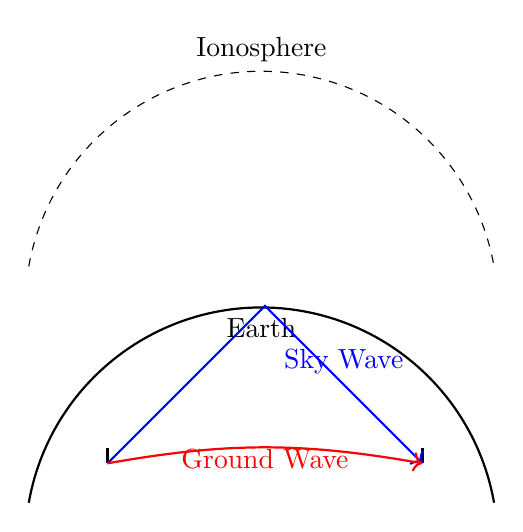
\begin{tikzpicture}
    % Earth
    \draw [thick] (-3, 0) arc (170:10:3) node [midway, below] {Earth};
    % Ionosphere
    \draw [dashed] (-3, 3) arc (170:10:3) node [midway, above] {Ionosphere};
    
    % TX RX
    \coordinate (TX) at (-2, 0.5);
    \coordinate (RX) at (2, 0.5);
    \draw [thick] (TX) -- +(0, 0.2);
    \draw [thick] (RX) -- +(0, 0.2);
    
    % Sky wave
    \draw [->, thick, blue] (TX) -- (0, 2.5) -- (RX) node [midway, above] {Sky Wave};
    
    % Ground wave
    \draw [->, thick, red] (TX) to [bend left=10] (RX);
    \node [below, red] at (0, 0.8) {Ground Wave};
\end{tikzpicture}
\end{answerdiagram}
\end{solutionbox}

\begin{mnemonicbox}
\mnemonic{"GIST" - Ground-Interface Surface Transmission vs Ionospheric Sky Transmission}
\end{mnemonicbox}

\questionmarks{5(a)}{3}{Explain three different types of Satellites}

\begin{solutionbox}
\begin{tabulary}{\linewidth}{|L|L|}
\hline
\textbf{Satellite Type} & \textbf{Characteristics} \\ \hline
\keyword{LEO} (Low Earth Orbit) & Altitude: 160-2,000 km, Period: ~90 min. Uses: Earth observation, comms. \\ \hline
\keyword{MEO} (Medium Earth Orbit) & Altitude: 2,000-35,786 km, Period: 2-24 hrs. Uses: Navigation (GPS). \\ \hline
\keyword{GEO} (Geostationary Orbit) & Altitude: 35,786 km, Period: 24 hrs. Uses: TV, Weather. \\ \hline
\end{tabulary}
\end{solutionbox}

\begin{mnemonicbox}
\mnemonic{"LMG" - Low Medium Geostationary}
\end{mnemonicbox}

\questionmarks{5(b)}{4}{What are smart antennas? Write two applications of it}

\begin{solutionbox}
Smart antennas are antenna systems that use digital signal processing algorithms to identify spatial signatures and dynamically adjust radiation patterns.

\begin{tabulary}{\linewidth}{|L|L|}
\hline
\textbf{Feature} & \textbf{Description} \\ \hline
\keyword{Types} & Switched beam systems, Adaptive array systems \\ \hline
\keyword{Operation} & Uses multiple antenna elements and signal processing to adapt \\ \hline
\keyword{Benefits} & Increased capacity, improved coverage, reduced interference \\ \hline
\end{tabulary}

\textbf{Applications:}
1. Mobile cellular networks (4G, 5G).
2. Wireless LANs (Wi-Fi).
\end{solutionbox}

\begin{mnemonicbox}
\mnemonic{"SMART" - Signal Manipulation And Response Technology}
\end{mnemonicbox}

\questionmarks{5(c)}{7}{What is Satellite communication? Explain Data Communication}

\begin{solutionbox}
\textbf{Satellite Communication} is the use of artificial satellites to provide communication links between various points on Earth.

\begin{answerdiagram}{Satellite Link}
\begin{tikzpicture}
    % Earth Stations
    \node [gtu block] (tx) {TX Earth Station};
    \node [gtu block, right=of tx, xshift=2cm] (rx) {RX Earth Station};
    
    % Satellite
    \node [draw, circle, minimum size=1.5cm, above=of tx, xshift=2.5cm, yshift=1cm] (sat) {Satellite};
    
    % Signals
    \draw [->, thick] (tx) -- node [left] {Uplink (6 GHz)} (sat);
    \draw [->, thick] (sat) -- node [right] {Downlink (4 GHz)} (rx);
\end{tikzpicture}
\end{answerdiagram}

\textbf{Data Communication via Satellite:}
\begin{tabulary}{\linewidth}{|L|L|}
\hline
\textbf{Component} & \textbf{Function} \\ \hline
\keyword{Earth Station} & Transmits/receives signals to/from satellites \\ \hline
\keyword{Transponder} & Receives, amplifies and retransmits signals at different frequencies \\ \hline
\keyword{Access methods} & FDMA, TDMA, CDMA to allow multiple users to share capacity \\ \hline
\keyword{Applications} & Internet backhaul, VSAT networks, IoT \\ \hline
\keyword{Advantages} & Wide coverage area, independence from terrestrial infrastructure \\ \hline
\end{tabulary}
\end{solutionbox}

\begin{mnemonicbox}
\mnemonic{"UPDATA" - Uplink Provides Data Access To All}
\end{mnemonicbox}

\orquestionmarks{5(a)}{3}{Write laws of Kepler for satellite}

\begin{solutionbox}
\begin{tabulary}{\linewidth}{|L|L|}
\hline
\textbf{Law} & \textbf{Description} \\ \hline
\textbf{First Law} & Satellites orbit in elliptical paths with the Earth at one focus \\ \hline
\textbf{Second Law} & A line joining the satellite and Earth sweeps out equal areas in equal times \\ \hline
\textbf{Third Law} & The square of the orbital period is proportional to the cube of the semi-major axis ($T^2 \propto a^3$) \\ \hline
\end{tabulary}
\end{solutionbox}

\begin{mnemonicbox}
\mnemonic{"ESP" - Elliptical orbits, Sweep equal areas, Period-distance relation}
\end{mnemonicbox}

\orquestionmarks{5(b)}{4}{Explain Base station and Mobile station antennas}

\begin{solutionbox}
\textbf{Base Station Antennas:}
\begin{itemize}
    \item \textbf{Types}: Omnidirectional, sector, panel antennas.
    \item \textbf{Gain}: Typically 10-18 dBi.
    \item \textbf{Mounting}: Tower or rooftop installation.
\end{itemize}

\textbf{Mobile Station Antennas:}
\begin{itemize}
    \item \textbf{Types}: Internal PIFA, patch, monopole.
    \item \textbf{Gain}: Low gain (0-3 dBi).
    \item \textbf{Size}: Compact, integrated inside device.
\end{itemize}

\begin{answerdiagram}{Base vs Mobile}
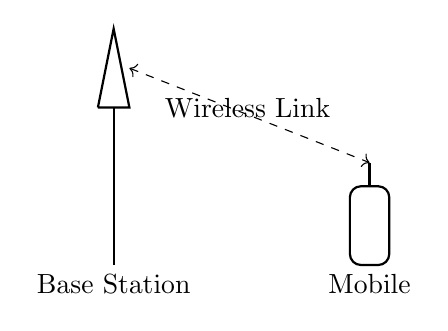
\begin{tikzpicture}
    % Base
    \draw [thick] (0,0) -- (0, 2);
    \draw [thick] (-0.2, 2) -- (0.2, 2) -- (0, 3) -- (-0.2, 2); % Tower top
    \node [below] at (0,0) {Base Station};
    
    % Mobile
    \draw [thick, rounded corners] (3, 0) rectangle (3.5, 1);
    \draw [thick] (3.25, 1) -- (3.25, 1.3);
    \node [below] at (3.25, 0) {Mobile};
    
    \draw [dashed, <->] (0.2, 2.5) -- (3.25, 1.3);
    \node at (1.7, 2) {Wireless Link};
\end{tikzpicture}
\end{answerdiagram}
\end{solutionbox}

\begin{mnemonicbox}
\mnemonic{"BIMS" - Base stations Install Multiple Sectors, Mobile stations Stay small}
\end{mnemonicbox}

\orquestionmarks{5(c)}{7}{Explain DTH receiver system in detail}

\begin{solutionbox}
\textbf{DTH (Direct-to-Home)} receiver system delivers television signals directly to users via satellite.

\begin{answerdiagram}{DTH System}
\begin{tikzpicture}[node distance=1.5cm]
    \node [draw, circle] (sat) {Satellite};
    \node [gtu block, below=of sat] (dish) {Dish Antenna};
    \node [gtu block, below=of dish] (lnb) {LNB};
    \node [gtu block, right=of lnb] (stb) {Set-top Box};
    \node [gtu block, right=of stb] (tv) {TV};
    
    \draw [->, dashed] (sat) -- (dish);
    \draw [gtu arrow] (dish) -- (lnb);
    \draw [gtu arrow] (lnb) -- node [above] {Cable} (stb);
    \draw [gtu arrow] (stb) -- (tv);
\end{tikzpicture}
\end{answerdiagram}

\begin{tabulary}{\linewidth}{|L|L|}
\hline
\textbf{Component} & \textbf{Function} \\ \hline
\keyword{Dish Antenna} & Parabolic reflector to collect satellite signals (45-90 cm) \\ \hline
\keyword{LNB} & Low Noise Block downconverter; amplifies signal and converts to lower frequency \\ \hline
\keyword{Set-top Box} & Decodes digital signals and converts to audio/video for TV \\ \hline
\keyword{TV} & Display unit \\ \hline
\end{tabulary}
\end{solutionbox}

\end{document}
